\documentclass[a4paper]{article}

\usepackage[french]{babel}
\usepackage[utf8]{inputenc}
\usepackage{amsmath}
\usepackage{graphicx}
\usepackage[colorinlistoftodos]{todonotes}
\usepackage[T1]{fontenc}
\usepackage{color}
\usepackage{fancyhdr}
\usepackage{MnSymbol,wasysym}
\usepackage{hyperref}
\pagestyle{fancy}

\fancyhead[c]{\textbf{Rapport rédigé par le groupe Brave Cowards Studio}}
\fancyhead[r]{}
\fancyhead[l]{}
\fancyfoot[c]{EPITA-Ecole d'Ingénieurs en Informatique}
\fancyfoot[l]{\today}
\fancyfoot[r]{page \thepage}

\title{\textbf{\huge Rapport \\ De \\ Soutenance }}

\author{DAUVERT-LATRE Max-Emilien (Chef de projet)\\ FOURREAU-HARDY Elie\\ GOYAT Nathan}

\date{\today}

\begin{document}

\maketitle
{\centering\Large Créé par les développeurs de \\ \textbf{\Huge Brave Cowards Studio}  \\ \Large en partenariat avec \\ \textbf{\huge UNITY} \\ 
\includegraphics[width=0.5\textwidth]{UNITY.jpg} \\ }

\pagebreak

\tableofcontents 

\pagebreak

\section{Introduction}
\vspace{0.5 cm}
Après plusieurs changements dans le groupe qui a été remodélisé 2 fois, nous nous retrouvons donc dans un groupe constitué de 3 personnes. Nous avons perdu 2 fondateurs du groupe originel, l'un qui a changé d'école sans prévenir et qui était de plus le chef de projet, et l'autre qui est passé en classe \#. Nous nous retrouvons donc à 2 et nous récupérons un autre groupe de 2 personnes qui au final ne sera qu'un groupe d'une seule personne. Notre groupe final est donc constitué de 3 personnes.\\ 
Depuis que nous avons fini de constituer le groupe, rechoisir un chef de projet et refaire de nouveau de le cahier des charges, nous nous sommes réunis plusieurs fois. Durant ces réunions nous avons discuté plus en détails du jeu en lui même et des différentes parties de son développement. Nous nous sommes ensuite répartis les tâches et nous avons commencé à travailler dessus. Ce rapport récapitule ce que nous avons fait pour le projet depuis le rendu du cahier des charges et l'emploi du temps que nous prévoyons tenir, que ce soit pour le gameplay, le développement des niveaux ou la physique du personnage et des différents éléments du monde autour.



\pagebreak

\section{Avancement : depuis le cahier des charges}

\textbf{Notes :}
\vspace{0.2 cm}

Toutes les notions abordées plus bas présentent le jeu dans son état actuel et ne reviennent pas sur ce qu'il était auparavant, car le groupe a démaré la création du jeu de zéro, après la création du cahier des charge.\\
Ne vous étonnez donc pas si la partie "Avancement" ressemble à une simple présentation complète qui décrit tout les aspects importants du jeu au moment de la première soutenance.
\\


\subsection{Le gameplay}
\vspace{0.5 cm}

Définissons tout d’abord le terme « gameplay ». Il s'agit de toutes les différentes actions que peut effectuer le joueur  pour intéragir dans le jeu, allant de la manière de se déplacer jusqu'aux objets utilisable en passant par les objectifs de jeu.\\
 \\
Dans l'état actuel, nous avons toutes les interactions basiques que l'on attend de ce type de jeu, à savoir celles d'un  jeu de plateforme et d'un jeu à la première personne.\\
\\
Dans un premier temps, nous avons le simple déplacement du personnage que l'on contrôle. En effet en pressant les touches appropriées, le personnage va pouvoir se déplacer dans différentes directions en fonction de là où il regarde (car le point de vue est celui de l'avatar, tout se base sur lui). A cela s'accompagne une caméra fonctionnelle représentant le regard du personnage. Et déplacer la souris nous permet alors d'orienter le regard du personnage  dans la direction que l'on souhaite.\\
\\
De ces contrôles basiques découlent alors deux autres interactions avec le personnage: la première est très importante à la fois pour un jeu à la première personne et pour un jeu de plateforme : il s'agit de sprinter. Cela va permettre au personnage d'augmenter de manière drastique sa vitesse de course et donc de pouvoir franchir plus facilement des précipices qui auraient été normalement impossible de franchir\\
\\
La seconde interaction est le fait de pouvoir s'accroupir. Cela va permettre au personnage, par exemple, de pouvoir passer en dessous d'obstacles situés à sa hauteur.\\
Enfin, il ne faut pas oublier le plus important, sans quoi le jeu ne serait pas un  jeu de plateforme, qui est bien sûr la capacité du personnage à sauter. Il s'agit se l'élément principal du gameplay et donc contrairement à un jeu de tir, où l'on améliore, par exemple, l'armement, c'est la capacité de saut qui sera améliorée tout au long de la progression du joueur (voir: Gameplay, seconde partie). Dans cette première version le saut est très simple et permettra simplement au personnage de passer de plateforme en plateforme.
\\

\pagebreak

Etant donné que nous avons affaire à un jeu qui va demander au joueur d’aller rapidement d'un point A à un point B en évitant plusieurs obstacles, le contrôle du personnage doit donc être instinctif, fluide et total. Nous avons donc décidé, comme dans beaucoup d'autres jeux, d'ajouter du \og air control \fg {}. Le principe est simple: le  \og air control \fg {} permet au joueur de contrôler les mouvements ainsi que la célérité du personnage même quand celui-ci ce trouve dans les airs, permettant de faire des sauts très précis, ce qui est essentiel. Dans la même idée le personnage saute plus haut qu'un humain normal, permettant à celui-ci de pouvoir atteindre des plateformes plus éloignées, rendant l'action plus impressionnante tout en gardant cette sensation de contrôle chez le joueur, qui est selon nous, très importante pour le confort de jeu.

\pagebreak

\subsection{Le niveau}
\vspace{0.5 cm}

L'univers dans lequel le personnage évolue est un archipel d'îles flottantes et il se trouve sur la plus basse de ces îles au début du jeu. C'est donc là que commence le premier niveau.\\
\\
 Le personnage se situe donc sur l'île volante à la base de l'archipel. Elle est petite en taille par rapport aux autres îles (qui ne sont pas encore présentes) et ne contient, à sa surface, qu'un mystérieux temple. Ce temple est composé de plusieurs piliers soutenant des blocs. Ils s'agit de la seule construction de l'île.
Le parcours de jeu est, pour le moment, composé de simples plateformes volantes, représentant différents rochers et débris gravitant autours de  l'îles. Le placement de ces rochers est très commode, puisqu'ils permettent au personnage de se trouver un chemin vers une île située plus en hauteur à l'aide de sauts bien effectués. Cette île plus en hauteur possède un temple semblable au premier.
Pour l'instant l'apparence des blocs composant le parcours est assez simpliste mais chaque objet possède une texture propre.\\
\\
Ce niveau est un parcours d'essai suffisant pour voir les capacités du personnage et un avant goût de l’univers du jeu.\\
\\
\\
\\

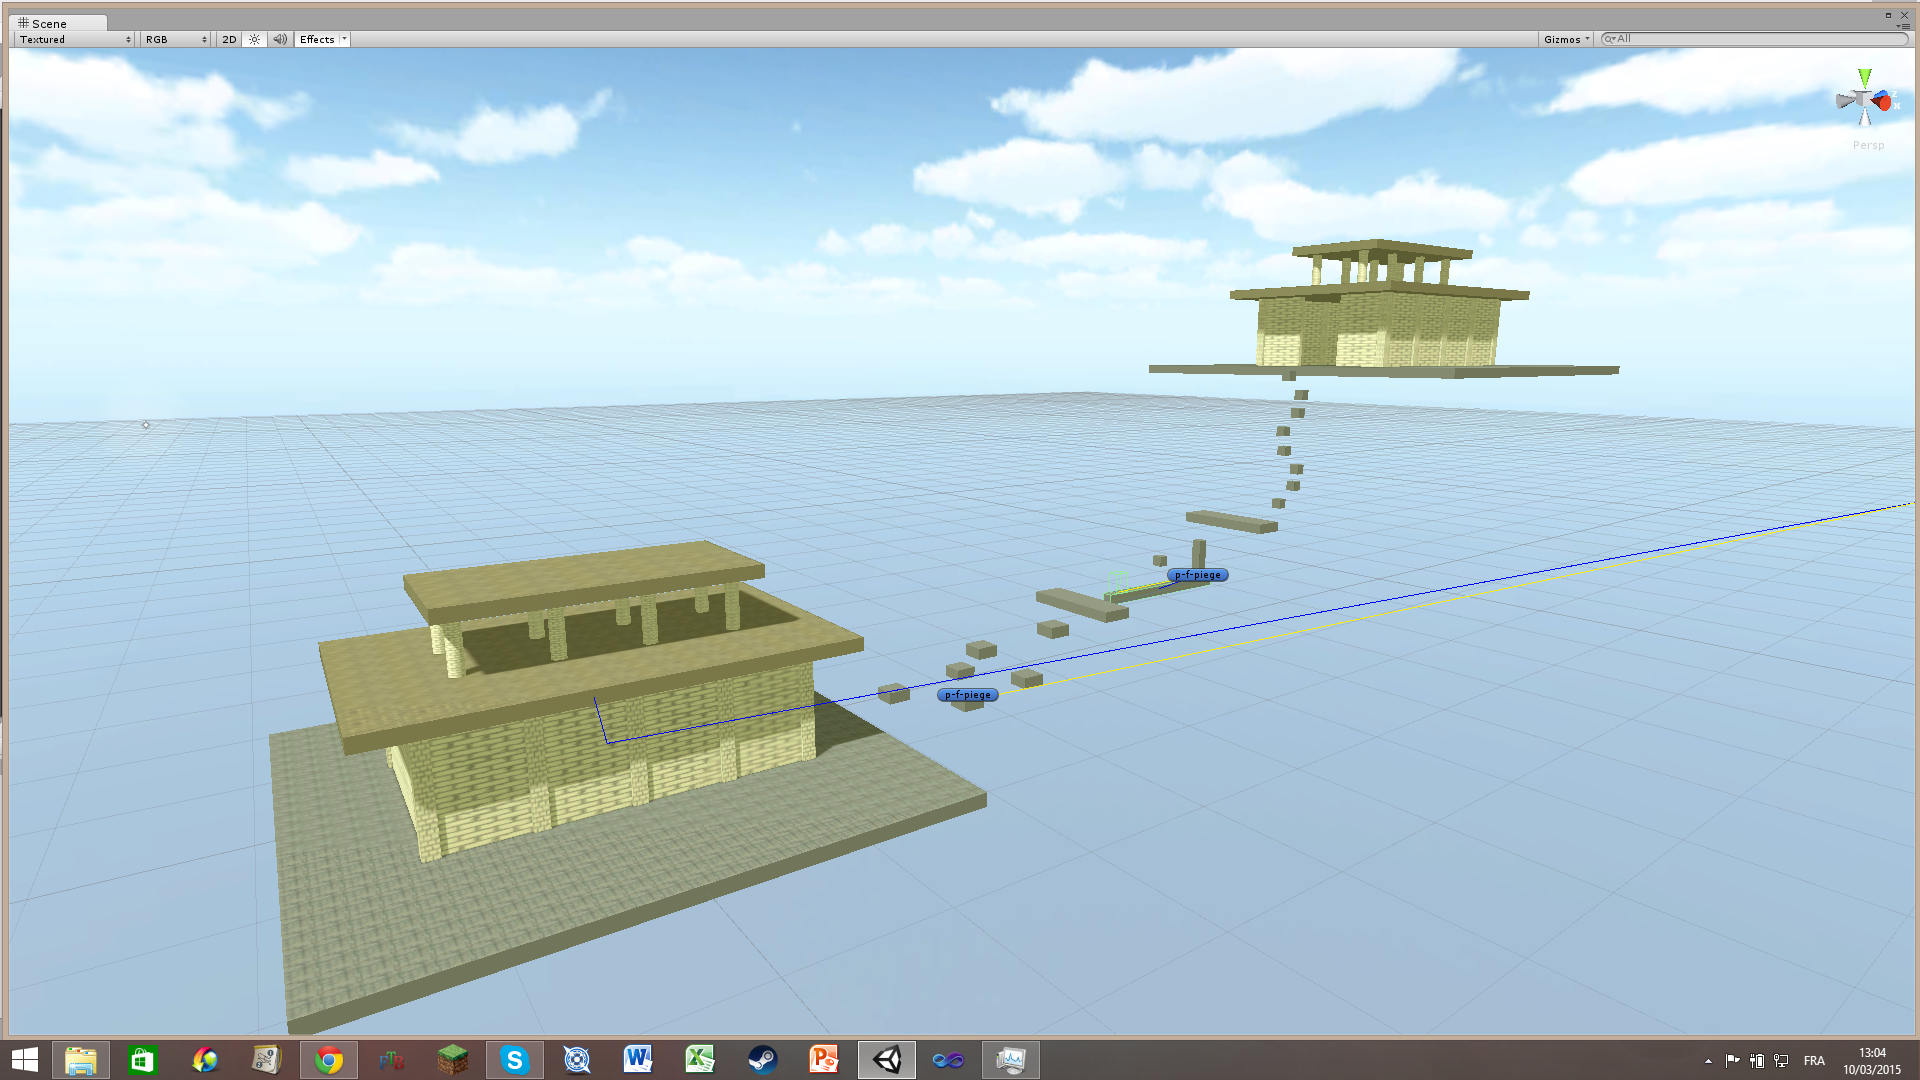
\includegraphics[width=1.1\textwidth]{parcour_lvl1_V1.png}


\pagebreak

\subsection{La physique}
\vspace{0.5 cm}

Entre toutes les choses sur lesquelles Unity nous facilite la tâche, c'est bien sûr la physique que l'on gagne le plus de temps.\\
La physique est un élément primordial pour créer un univers de jeu cohérent, surtout si l'on donne à l'univers du jeu des règles semblables à celles du monde dans lequel on vit, ce qui semble le meilleur choix pour que le joueur ne soit pas trop perdu une fois dans le jeu, car il y retrouve un univers familier.
Ces \og règles \fg {} se manifestent par plusieurs aspects physiques qui sont donc incorporés dans le jeu avec plus ou moins de variables par rapport à la réalité.\\
\\
-La gravité: Si les différentes îles présentes dans le jeu (voir partie: niveau) semblent être soumises à une magie qui les immunise à cette force, elle s'applique cependant au personnage principal. En effet, ne rien avoir sous ses pieds ou perdre toute l’énergie dû à l'impulsion d'un saut fera irrémédiablement chuter le personnage vers une mort certaine... ou le sol d'une île.\\
\\
-Collisions: Jusqu’à preuve du contraire, le personnage principal n'est pas un fantôme, le fait de renter dans un mur causera donc l'arrêt de tous ses mouvements. Il serait, en effet,  dommage que le personnage passe au travers de la plateforme sur laquelle il était censé atterrir.\\
\\
-Interaction : En entrant en contact avec certains objets, le joueur va pouvoir déclencher des actions qui lui permettront d'avancer dans le jeu. Une action pourrait être, par exemple, de passer au niveau suivant ou d'activer des objets.\\
\\
-Éclairage : Unity nous permet d'avoir un éclairage dynamique, créant des zone d'ombres en fonction de la position des bâtiments ou objets et de la position du soleil.


\pagebreak

\subsection{Avance/Retard pris}
\vspace{0.5 cm}


Jetons désormais un petit coup d’œil au planning pour voir point par point, en reprenant ce que l'on a dit précédemment  si cette version présentée pour cette première soutenance est conforme à la limite de temps que nous nous sommes fixés:\\
\\
Le gameplay est exactement au point où on le souhaitait, le personnage est capable  faire le parcours de saut simple que l'on a créé. C'est donc un parfait point de départ pour rajouter toute sorte d'améliorations qui enrichirons le jeu.\\
\\
L'avancement du niveau est peut-être légèrement en dessous de ce que l'on avait prévu. En effet, on veut donner à l'exploration une certaine importance dans le jeu. Or le niveau actuel n'est qu'un parcours de plateformes. Nous sommes satisfaits de ce parcours, mais on dirait bien que l'île à explorer est reportée pour la prochaine soutenance.\\
\\
On ne le dira jamais assez, Unity nous facilite vraiment la tâche pour la physique est comme dit plus bas tout est maintenant question d'optimisation et les légères modifications seront faites selon nos besoins, en soit, on peut dire que l'on est en avance sur ce point là.\\
\\
En soit on peut dire que le retard que l'on a pris sur le level-design se rattrape sur le travaille du personnage et de la physique, en se repartissant bien les tâches, de telle sorte  que des personnes travaillent uniquement sur le niveau et d'autres travaillent sur les ajouts au gameplay on pourra créer un niveau très intéressant à jouer autant au niveau du level-design que du gameplay.


\pagebreak

\section{Prévisions : La prochaine soutenance}
\vspace{0.5 cm}

\subsection{Le gameplay}
\vspace{0.5 cm}

Pour la prochaine soutenance l'une des meilleures améliorations que nous pouvons apporter au jeu se situe dans le gameplay. En effet nous partons d'un principe des plus simples, celui d'un jeu de plateforme. Or, la seule restriction qui permet de définir un tel genre de jeu est la suivante: il faut partir d'un point A (début du niveau) et arriver à un point B tout en évitant différents obstacles. Et le chemin que l'on devra emprunter nécessitera de sauter d'une plateforme à une autre. 
Peu de choses sont donc nécessaires et on pourrait déjà dire que notre jeu répond à ces critères. Cependant pour enrichir notre jeu, le rendre plus intéressant et amusant, nous avons prévu de le démarquer en rajoutant des possibilités via le gameplay. \\
\\
Nous comptons tout d'abord ajouter un double-saut, c'est un principe simple qui remonte à très loin dans l'histoire des jeux de plateforme: il s'agit de permettre au personnage de se donner une nouvelle impulsion une fois dans les airs. Cela va donner une toute nouvelle dimension au jeu, car le personnage pourra alors passer de tous nouveaux obstacles, qu'ils soient, plus loin, plus élevés ou nécessitent un changement de direction en l'air. Il ne sera pas disponible au tout début pour que le joueur puisse se familiariser avec les sauts normaux, et sera justifié par un certain objet.\\
\\
Nous ajouterons ensuite des interactions avec le décor. Certains endroit dans le niveau pourrons, par exemple, servir de tremplins qui le projetteront dans les airs, et cela bien plus haut qu'un saut. Il s'agira, à plusieurs endroits dans le jeu, du seul moyen pour progresser.\\
\\
Il est également possible que des objets utilisables soient rajoutés. Le personnage les portera sur lui et pourra les utiliser dès qu'il le souhaitera, mais ils ne sont encore qu'à l'état de concept. Il pourrait, d’ailleurs, ne pas s'agir d'objets mais de capacités que le personnage acquerra au long du jeu.
L'un pourrait le faire sauter plus haut, l'autre lui faire parcourir une certaine distance dans les airs. Les possibilités sont infinie s.

\pagebreak

\subsection{Le niveau}
\vspace{0.5 cm}

Le niveau que l'on proposera pour la prochaine soutenance sera d'une toute autre échelle. En effet, nous souhaitons créer la première île principal. Elle sera bien plus grande que les deux îles présentes dans le niveau de la première soutenance. Elle ne pourra pas ainsi être balayée par un simple regard du personnage. Une partie d'exploration sera alors de mise pour découvrir tous ses secrets et, éventuellement la suite du jeu.
Les différentes variations de relief permettront d'incorporer le plus naturellement possible d'autres parcours de plateforme. Le fait que ces parcours soient directement à la surface de l'île les rendront moins... mortels, littéralement.\\
\\
Entre autres, la diversité graphique sera aussi vue à la hausse. Le niveau de la première soutenance contient en soi très peu de textures, par conséquent le nombre d'objets possédant des texture sera augmenté. Différents éléments de décors seront également ajoutés pour rendre l’ensemble plus riche et plus vivant . Par exemple, des arbres, des rochers et autres.\\
\\
On aura donc une île digne de ce nom qui sera la vraie base de l'aventure dans laquelle le joueur se lancera. En effet le niveau présenté à la première soutenance sert plus de tutoriel qu'autre chose. Avec cette seconde île, l'univers pourra vraiment se mettre en place et les nouvelles possibilités de gameplay pourront être pleinement exploitées. 


\pagebreak

\subsection{La physique}
\vspace{0.5 cm}

Comme dit lors de la première partie consacrée à la physique, Unity nous permet de gagner beaucoup de temps sur cette question en gérant par lui même beaucoup de moteurs physiques. Toutes les améliorations possible au niveau de la physique vont donc résider dans plusieurs choses, à savoir l'optimisation et la personnalisation.\\
\\
Pour la prochaine soutenance, nous avons donc prévu d'améliorer certains points déjà présents. Mais pour la plupart ils resteront très peu changés.  \\
Les collisions fonctionnent et, hormis certaines interactions spécifiques, devraient fonctionner de la même manière pour une grande partie des objets du jeu.\\
\\
L'éclairage, également, fonctionne bien et ne souffrira d'aucun changement, il s'agira surtout d'optimisation (rendre certaines ombre plus nette par exemple).\\
\\
La gravité, quant à elle, sera très certainement soumise au changement les plus importants. La manière dont le personnage  retombe, à quelle vitesse, le temps qu'il reste en l'air, à quelle hauteur il saute, sont tous des manifestations de l'effet de la gravité sur le personnage. Et la changer remet totalement en question la difficulté ou la possibilité de phase de plateforme. Comme ces phases sont pour l'instant peu nombreuses, on peut donc encore envisager de gros changements.\\
\\
Enfin, le son fera son apparition à la seconde soutenance, que ce soit des bruitages ou une musique de fond. Ils accompagneront le joueur dans son expérience de jeu.

\pagebreak

\subsection{Avance/Retard prévu}
\vspace{0.5 cm}

Essayons maintenant de prévoir où nous en serons lors de la prochaine soutenance et des éventuels retard que nous pourrions prendre. Ce ne sont donc que de pures suppositions mais elles seront utiles lors de la seconde soutenance. On pourra donc voir si on a tenu le planning et si les prévisions étaient bonnes.\\
\\
Dans un premier temps essayons de voir ce que pourrait donner le niveau lors de cette seconde soutenance. Je pense que cette fameuse île principale sera forcemment présente car il s’agit de l'élément central du premier niveau. Là où l'on va voir des variations, c'est au niveau de la diversité de ce que l'on va trouver sur l'île. Plus on sera en avance, plus les décors, parcours et textures seront travaillés. Au contraire, si on est en retard, il n'y aura que le strict minimum.\\
\\
De même, les avancés de gameplay seront variables en nombres. Le double saut et les éléments du décors qui nous projettent en l'air seront, par exemple, forcemment là. Mais si le gameplay est très diversifié, ce sera une preuve que l'on a pris de l'avance à ce niveau.\\
\\
Enfin, je ne pense pas que l'on puisse avoir du retard sur la physique, car nous pensons vraiment que la plus grande partie du travail a été faite sur ce point. Il est donc même très probable que tous ce qui est en rapport avec la physique du jeu soit finalisé à la seconde soutenance.\\
\\
On a donc plus ou moins des prévisions semblables au premier point sur le retard et l'avance du rapport, à savoir que le level-design sera peut-être le plus en retard mais que le reste compensera.

\pagebreak


\section{L'expérience de création de l'équipe}
\vspace{0.3 cm}

\textbf{L'équipe de Braves Cowards Studio vous parle de leur ressentis lors de la création du projet jusqu'à maintenant.}
\\


\subsection{DAUVERT-LATRE Max-Emilien}
\vspace{0.5 cm}

Mon rôle pour cette première soutenance était de créer le menu du jeu partiellement et principalement le côté esthétique de notre premier niveau de jeu, c’est-à-dire que je devais mettre en place certaines textures ainsi que la mise en forme du niveau. \\Premièrement j’ai commencé par rechercher les renseignements de base sur la création d’un menu, après cela je me suis attelé à réaliser en premier lieu un fond de menu qui soit dans l’idée de notre jeu. Je cherchais donc un fond représentant le ciel que j’ai trouvé dans les presetting de UNITY.\\Voici le fond de base vu par la caméra intégrée de UNITY :\\ \\ \\ \\ \\
\begin{figure}[h]
\begin{center}
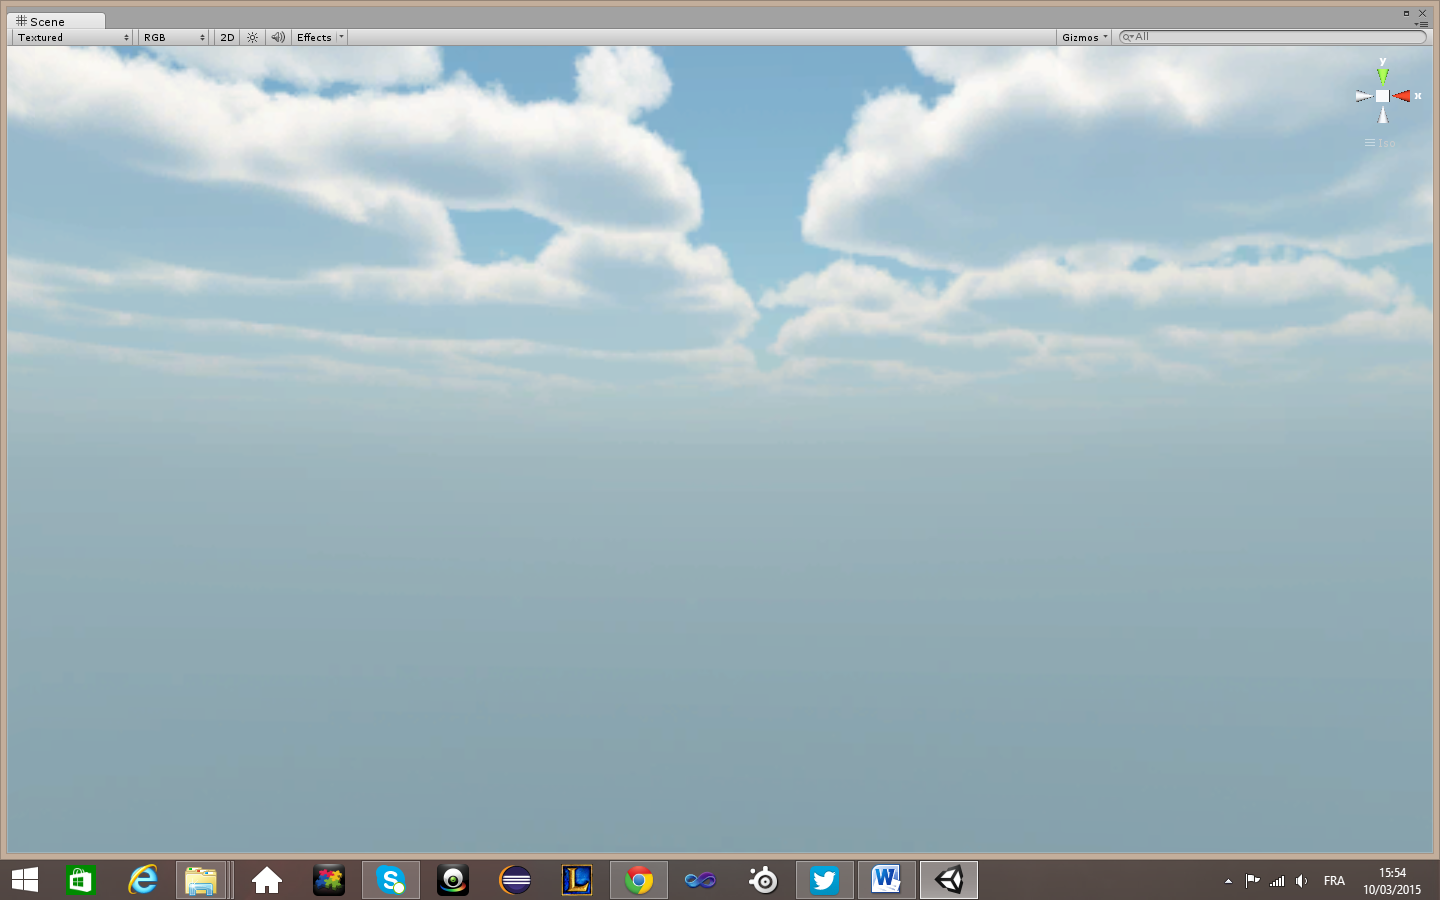
\includegraphics[width=1\textwidth]{sky1.png}
\end{center}
\end{figure}

\pagebreak
L’image étant trop sombre et pas à mon goût, j’ai joué avec la rotation de la caméra pour obtenir une vision plus haute du ciel ainsi qu’une vue sur le soleil :
\begin{figure}[h]
\begin{center}
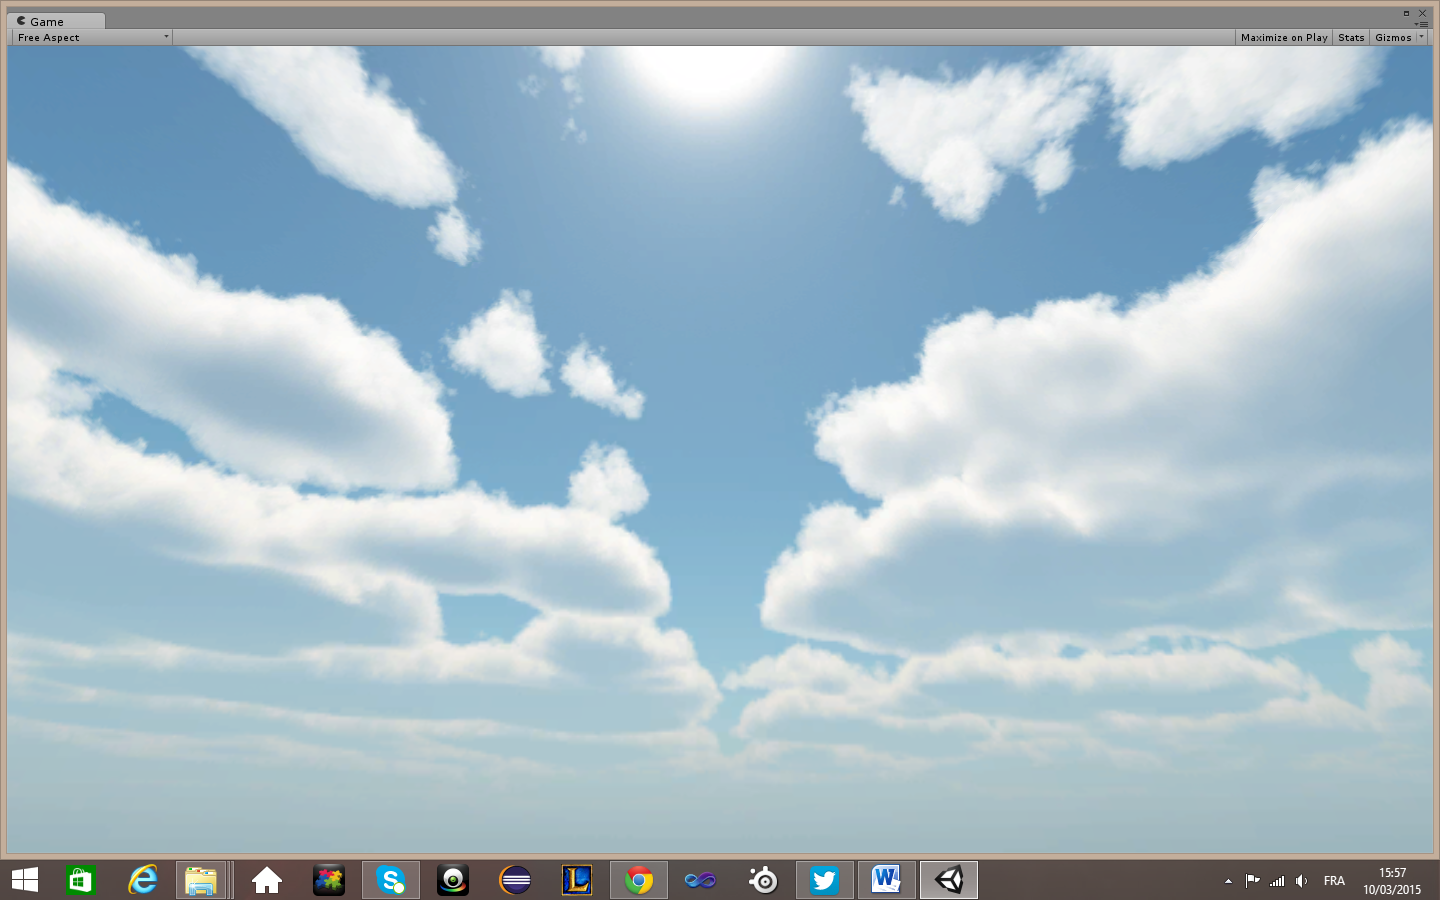
\includegraphics[width=1\textwidth]{sky2.png}
\end{center}
\end{figure}
Il ne me reste plus qu’à écrire le menu et faire les interactions de base.\\
	Le menu est constitué de l’affichage du titre du jeu centré suivi des différents boutons. J’ai fait le titre d’une couleur qui ressors du décors, rouge mais j’ai diminuer la composante alpha afin de l’écrire de façon plus translucide. Les autres options sont dans l’ordre NOUVELLE PARTIE, CONTINUER, OPTIONS, CREDITS, AIDE, écrits dans un bleu opaque. J’ai réglé par le biais de UNITY les effets sur les boutons quand la souris passe dessus ou est cliqué.
    
\begin{figure}[h]
\begin{center}
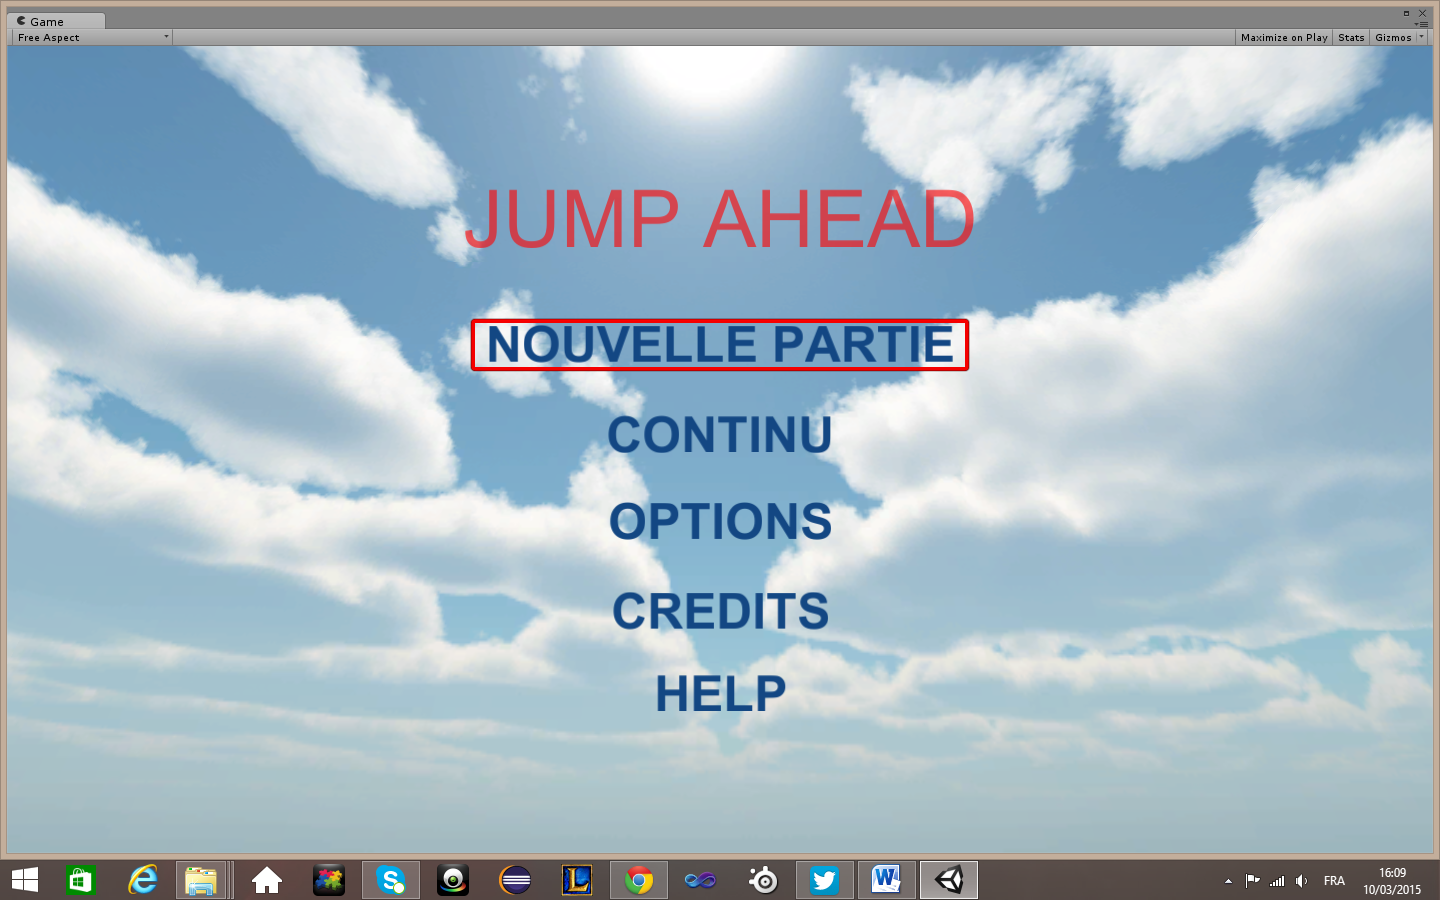
\includegraphics[width=0.95\textwidth]{menu1.png}
\end{center}
\end{figure}
PROBLEMES RENCONTRES :\\
Bien que les exacts même réglages soient faits pour les boutons, la couleur lors du passage de la souris sur le bouton est différentes entre les deux premiers et les 3 derniers, il semble que les 3 derniers boutons aient une teinte de différence dans le rouge alors que la palette indique la même couleur. Il se peut que se soit dû à l’inclinaison de la caméra.\\
Il ne reste plus que les interactions lors du clique. J’ai codé un programme qui lance sur une nouvelle scène qui dépend de l’architecture du projet ainsi l’appui sur NOUVELLE PARTIE vous emmène à la scène numéro 1 dans la hyérarchie du projet, ici le niveau 1.\\ 

\begin{figure}[h]
\begin{center}
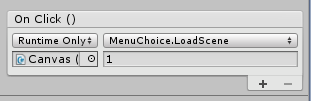
\includegraphics[width=1\textwidth]{fonctionClick.png}
\end{center}
\end{figure}

\begin{figure}[h]
\begin{center}
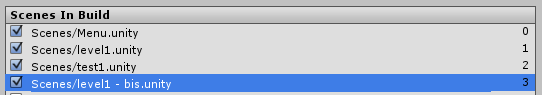
\includegraphics[width=1\textwidth]{build.png}
\end{center}
\end{figure}

Le menu n’est qu’opérationnel que pour le niveau 1. Nous n’avons pas encore défini les options ou la fonction de sauvegarde du bouton CONTINUER.\\



\textbf{ Menu pour la prochaine soutenance : }
\begin{itemize}
\item[-]Régler le problème couleur du menu 
\item[-]Installer une musique de fond
\item[-]Mettre quelques éléments dynamiques en fond
\item[-]Finir les parties OPTIONS, CREDIT et AIDE
\end{itemize}

\pagebreak
La suite de mon travail était la réalisation du spawn du jeu pour ne pas avoir qu’une simple plateforme. Le jeu se déroulant dans le ciel, j’ai décidé de prendre les couleurs assez claires proche du beige, voire blanc. La couleur n’étant pas la seule chose importante, il faut aussi une texture. Nous avons choisi un style rocailleux, avec des briques et une architecture proche de temples grecques pour le bâtiment du spawn :  

\begin{figure}[h]
\begin{center}
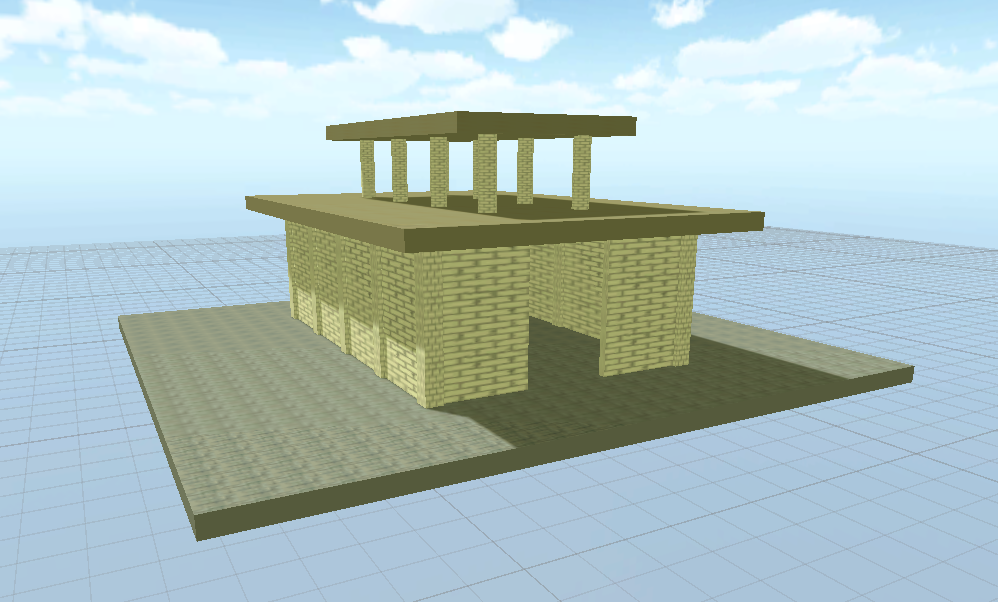
\includegraphics[width=1\textwidth]{spawn.png}
\end{center}
\end{figure}
\textbf{PROBLEMES RENCONTRES :}
Un problème visible ici est le fait que pour un objet avec une texture réglée convenablement avec la taille et le ratio, ici les piliers, si je mets la même texture pour des objets autres ( voir les murs reliants les piliers ), les ratios ne changent pas, donnant des briques trop grandes et allongées. Le ratio semble être un paramètre héréditaire de la texture, si je change le ratio pour les murs alors les piliers auront à leur tour le problème de ratio.\\
De base sur UNITY, il existe 2 types d’ombre, les statiques et les dynamiques, pour ne pas demander au jeu de calculer à chaque frame les ombres d’un même objet alors qu’il est statique, j’ai défini tout les objets non dynamiques en « static » afin de pouvoir faire un Lightmapping. C’est un fichier associé à la scène qui raffine les ombres des objets statiques en spécifiant au processeur qu’il n’a pas besoin de les recalculer, économie de mémoire et moins de latence. L’ombre du personnage sera très différente car elle est dynamique ( plus sombre ).
\\ \\ \\
\textbf{Pour la prochaine soutenance :}
\begin{itemize}
\item[-]Régler le problème des textures
\item[-]Rendre le spawn plus courbé et détaillé, moins brute de fonderie
\item[-]Gérer les textures de tous les préfabs déjà établis
\item[-]Création d’autres bâtiments et de designs
\end{itemize}

\pagebreak
J'ai en parallèle réalisé notre site Internet par le biais d'un site de création de page Internet \href{http://manager.e-monsite.com/site/welcome/begin}{e-monsite} qui m'a permi de créer facilement un site fonctionnel qui comprend de multiples plugins tels que l'agenda, le livre d'or ou encore les forums de discussion. Le site offre aussi un système d'inscription et une interface administrative complète. Le site est à l'adresse :\\
\url{http://brave-cowards-studio.e-monsite.com}



\pagebreak


\subsection{GOYAT Nathan}
\vspace{0.5 cm}


Comme je n’avais jamais utilisé Unity avant le début du projet ou un logiciel équivalent, j’ai eu beaucoup de mal à commencer. Heureusement, j’ai regardé pas mal de tutoriels pour m’aider et j’ai rapidement pris le coup de main.\\
Mon rôle était de créer des objet avec lesquels le joueur pourrait interragir.\\
J'ai alors commencé par créer des objets de tests pour me familiariser avec Unity. J'ai alors modifier les paramètres et composantes des objets pour bien comprendre leur fonctionnement. Une fois bien familiarisé avec, j'ai commencé à faire des objets qui pourront être utilisés dans les niveaux du jeu. J'ai créé des interrupteurs, des plateformes normales, des plateformes qui tombent et d'autres objets qui sont encore en développement. Mais au moment de l'écriture du script qui permettra au joueur de déclencher les actions des objets concernés j'ai eu de gros problèmes. L'utilisation de la fonction associée nécessitait plusieurs conditions que je ne connaissais pas au début. Je suis alors allé sur de nombreux sites pour me renseigner et j'ai fini par trouver la solution.\\
Mais pour l'appliquer, il m'a fallut modifier le personnage, et cela a produit de gros problèmes sur lui. Le joueur s'envolait, tombait ventre à terre, sans que le joueur ait fait ou ne puisse faire quoi que ce soit. J'ai alors élaboré un système alternatif mais il n'était pas concluant alors je l'ai abandonné. J'ai fait une recherche pendant plusieurs jours pour trouver une nouvelle alternative qui permette de détecter les collisions entre objets, mais elle s'est révélée infructueuse.\\
J'ai alors eu une discution avec mon groupe. Suite à celle-ci, j'ai décidé de changer mon fusils d'épaule. Désormais, j'utilise un autre système, la détection d'entrée dans une zone. Comme je n'utilise plus la détection de collision mais la détection d'entrée en zone, je n'ai pas à modifierle personnage donc il n'a plus de problème. Cela est plus compliqué à faire (je dois créer tous les objets en deux fois) mais ce système à aussi des avantages. Il supprime des composants sur les objets et donc également des calculs qui sont inutiles. \\



\pagebreak


\subsection{FOURREAU-HARDY Elie}
\vspace{0.5 cm}

Lorsque le groupe a été reformé j'ai été le dernier à me mettre sérieusement sur Unity, et il se trouve qu'en programmation comme en utilisation de logiciel, j'ai toujours été, pas mauvais, mais légèrement plus lent à comprendre, ainsi le groupe avait toujours de l'avance sur ce qu'on faisait sur le projet par rapport a moi. \\
\\
Il faut le dire, aussi pratique que Unity soit pour tout ce qu'il nous économise de faire pour la réalisation d'un jeu, il n'en reste pas moins complexe. Se lancer sur un tel logiciel en autodidacte était très certainement plus dur que je ne l'avais imaginé.\\
\\
Lors des nombreuses fois où l'on s'est réuni avec le groupe pour savoir ce que l'on pourrait bien ajouter, ou quelle direction prendrais le jeu, j'ajoutais toujours mon petit grain de sel, car ayant du mal sur les mêmes points qu'eux sur Unity je savais de quoi ils était capables. Je testais beaucoup les niveau pour leur indiqué les chose a modifier, j'ai beaucoup influencé la forme qu'a pris le niveau aujourd'hui. Dans un sens c'est normal car je suis même la personne à l’initiative de la création de ce type de jeu dans ce type d'univers. Mais dès qu'un de mes camarades se confrontait a un problème, il trouvait la solution à celui-ci bien avant que je puisse l'aider.\\
\\
En définitive je pense que j'ai désormais fait mes armes, et on ne sera pas trop de 3 pour travailler sur le niveau ambitieux que nous avons prévu pour la seconde soutenance.

\pagebreak

\section{Conclusion}
\vspace{0.5 cm}

Avec l'approche imminente de cette première soutenance, nous sommes plutôt fière de nous. En effet malgré des changements importants dans le groupe qui sont arrivés tard s'il on compare la date de création du groupe et celle du changement, on peut tout de même dire que le groupe baigne dans une ambiance générale de travail de bonne volonté et d'entraide qui présage beaucoup de bien pour la suite.\\
On peut même espérer que la motivation aille grandissante au  fur et à mesure que le jeu évolue dans tout ce qu'il le compose, à savoir le gameplay ou l'univers.\\
Nous avons donc réussi à faire une version qui représente parfaitement à la fois tous le potentiel de notre jeu et ce que la version finale pourra donner.  




\end{document}










